\section{Numerical experiments}
We carry out numerical experiments for the Nonstationary Compressible Euler equations. On these examples we want to demonstrate the combination of $hp$-DG and Dynamical meshes.
The purpose of the first of the two examples presented is to verify the method and its ability to capture shock waves in flows in high Mach number regimes. In all numerical experiments, we consider the CFL stability condition of the form
\be
\tau_k\max_{K_i\in\mc{T}_h}\frac{1}{|K_i|}\lo\max_{j\in S\lo i \ro} |\Gamma_{ij}|\lambda_{\mc{P}\lo\bs{w}_h^k|_{\Gamma_{ij}}, \bs{n}_{ij}\ro}^{\max}\ro\leq CFL.
\ee
Here, $CFL$ is a given constant and $\lambda_{\mc{P}\lo\bs{w}_h^k|_{\Gamma_{ij}}, \bs{n}_{ij}\ro}^{\max}$ is the maximum over $\Gamma_{ij}$ of the spectral radius of the matrix $\mc{P}\lo\bs{w}_h^k|_{\Gamma_{ij}}, \bs{n}_{ij}\ro$.
\paragraph{}
Also in all numerical experiments, we consider the medium in which we study the flow to be air, and therefore we set $\kappa = 1.4$.
\paragraph{}
In the light of~\ref{sec:bnd}, the prescribed boundary states are derived from primitive variables denoted as $\rho_{EXT}, v_{1_EXT}, v_{2_{EXT}}, p_{EXT}$ using the transformations to the conservative variables.

\subsection{Flow in a channel}
These examples demonstrate transonic flows with high Mach numbers, where applying of shock capturing is crucial.
\subsubsection{Reflected shock benchmark}
This is a classic benchmark for the solution of compressible flow described in~\cite{reflected}.
The prescribed relative tolerance $TOL$ for guiding the $hp$-adaptivity was set to $0.5\%$.
There are two different prescribed boundary states for two inflow regimes, corresponding to the left (denoted with $^{LEFT}$), and to the top (denoted with $^{TOP}$) part of the boundary, and are derived from the following prescribed values
\begin{eqnarray}
\rho_{EXT}^{LEFT} & = & 1.0 \\
v_{1_{EXT}^{LEFT}} & = & 2.9 \\
v_{2_{EXT}^{LEFT}} & = & 0.0 \\
p_{EXT}^{LEFT} & = & 0.714286 \\
\\
\rho_{EXT}^{TOP} & = & 1.7 \\
v_{1_{EXT}^{TOP}} & = & 2.619334 \\
v_{2_{EXT}^{TOP}} & = & -0.5063 \\
p_{EXT}^{TOP} & = & 1.52819.
\end{eqnarray}
The initial state is chosen to be the one prescribed on the left part of the boundary (denoted with $^{LEFT}$).
The bottom part of the boundary is a solid wall, and the right part is outflow, with respective corresponding boundary conditions.
In the solution of this problem, we employed the shock capturing scheme described in~\ref{sec:vertex_limiter}.

In Figs.~\ref{fig:rs-1} -~\ref{fig:rs-4}, the solution and corresponding meshes with polynomial degress differentiated by the color, at various time levels are shown.

\begin{figure}[H]
\begin{center}
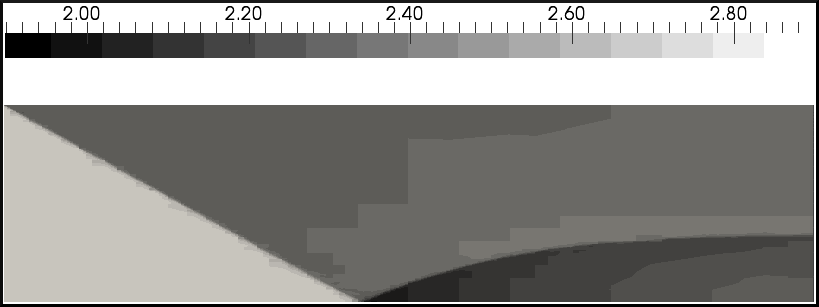
\includegraphics[width=\textwidth]{examples_img/reflected-shock/rs_sln.png}\ \ \ 
\end{center}

\caption{Solution: Mach number distribution, time = 1.0486s.}

\label{fig:rs-1}
\end{figure}

\begin{figure}[H]
\begin{center}
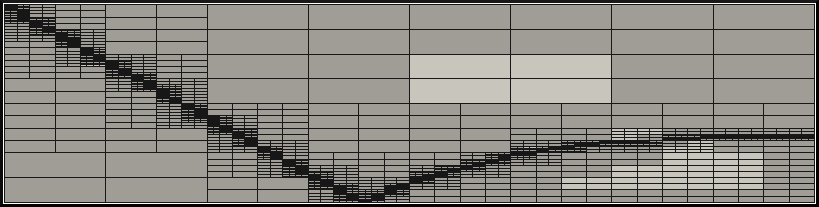
\includegraphics[width=\textwidth]{examples_img/reflected-shock/rs_mesh.png}\ \ \ 
\end{center}

\caption{Mesh, time = 1.0486s, number of DOFs: 17156.}

\label{fig:rs-2}
\end{figure}

\begin{figure}[H]
\begin{center}
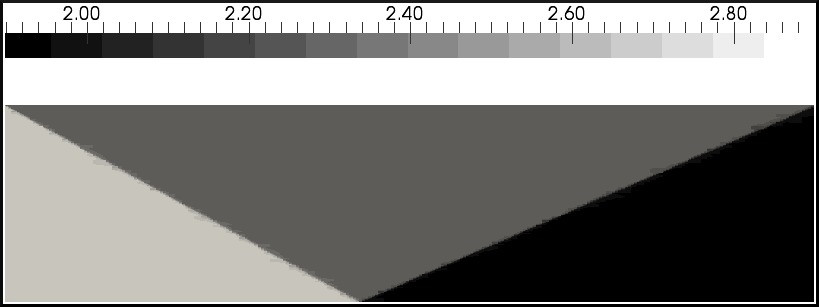
\includegraphics[width=\textwidth]{examples_img/reflected-shock/rs_finalSln.png}\ \ \ 
\end{center}

\caption{Final solution: Mach number distribution.}

\label{fig:rs-3}
\end{figure}

\begin{figure}[H]
\begin{center}
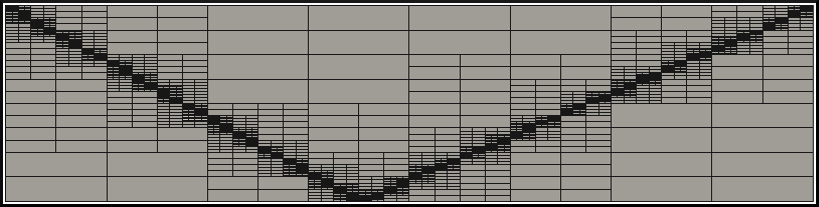
\includegraphics[width=\textwidth]{examples_img/reflected-shock/rs_finalMesh.png}\ \ \ 
\end{center}

\caption{Final mesh, number of DOFs: 30184.}

\label{fig:rs-4}
\end{figure}

In Fig.~\ref{fig:rs-11}, the same comparison to the exact solution, as in~\cite{reflected} was carried out, with good results.
\begin{figure}[H]
\begin{center}
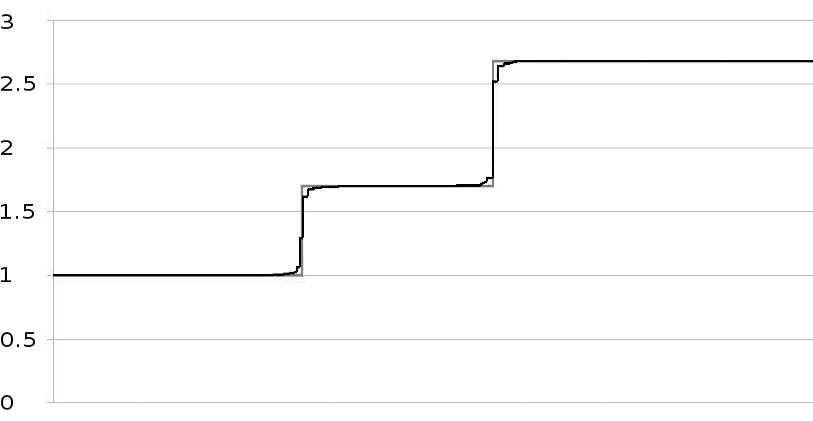
\includegraphics[width=\textwidth]{examples_img/reflected-shock/density.png}\ \ \ 
\end{center}

\caption{Density along the line y = 0.25, exact solution (light), and calculated solution (dark). See~\cite{reflected}, Fig. 4, for comparison}

\label{fig:rs-11}
\end{figure}	

\subsubsection{Forward facing step}
This is a classic benchmark for the solution of compressible flow.
In the light of~\ref{sec:bnd}, the prescribed boundary state is derived from the following prescribed values.
\begin{eqnarray}
\rho_{EXT} & = & 1.4 \\
v_{1_{EXT}} & = & 3.0 \\
v_{2_{EXT}} & = & 0.0 \\
p_{EXT} & = & 1.0
\end{eqnarray}
The left part of the boundary is an inlet part, whereas the right part is an outlet. The rest of the boundary is formed by solid walls.
The initial state is chosen to be the one prescribed on the left part of the boundary.
In the solution of this problem, we again employed the shock capturing scheme described in~\ref{sec:vertex_limiter}.
The prescribed relative tolerance $TOL$ for guiding the $hp$-adaptivity was set to $3.0\%$, later decreased to $2.0\%$ to capture the solution development.
In Figs.~\ref{fig:ffs-1} -~\ref{fig:ffs-4}, the solution and corresponding meshes with polynomial degress differentiated by the color, at various time levels are shown.

\begin{figure}[H]
\begin{center}
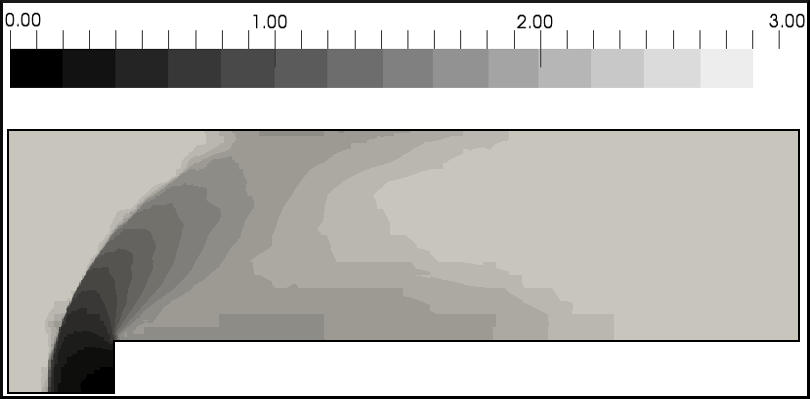
\includegraphics[width=0.7\textwidth]{examples_img/forward-step/sln1.png}\\
\vspace{2mm}
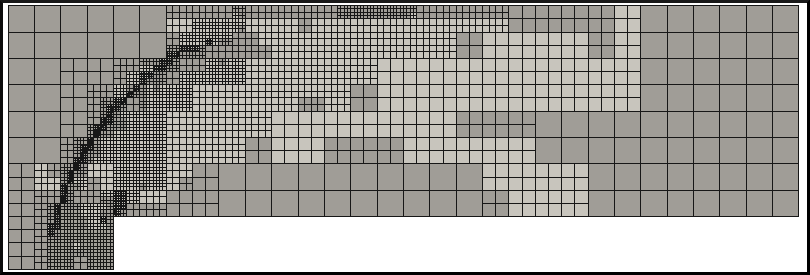
\includegraphics[width=0.7\textwidth]{examples_img/forward-step/mesh1.png}
\end{center}

\caption{Solution (Mach number distribution), and mesh, time = 0.616281.}

\label{fig:ffs-1}
\end{figure}

\begin{figure}[H]
\begin{center}
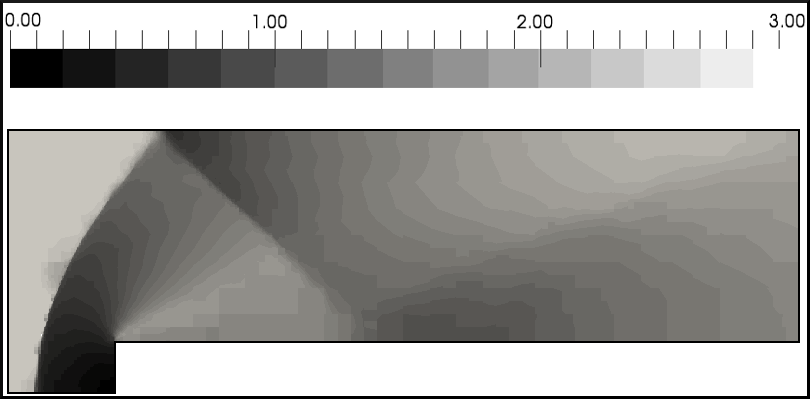
\includegraphics[width=0.7\textwidth]{examples_img/forward-step/sln2.png}\\
\vspace{2mm}
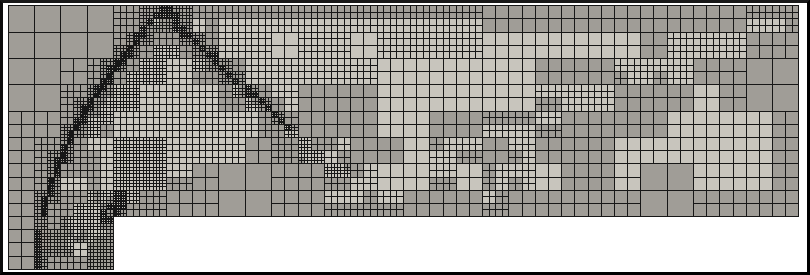
\includegraphics[width=0.7\textwidth]{examples_img/forward-step/mesh2.png}
\end{center}

\caption{Solution (Mach number distribution), and mesh, time = 2.07892.}

\label{fig:ffs-2}
\end{figure}

\begin{figure}[H]
\begin{center}
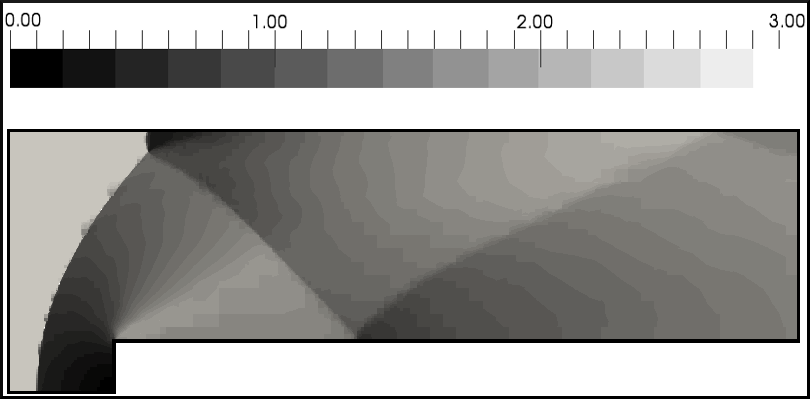
\includegraphics[width=0.7\textwidth]{examples_img/forward-step/sln3.png}\\
\vspace{2mm}
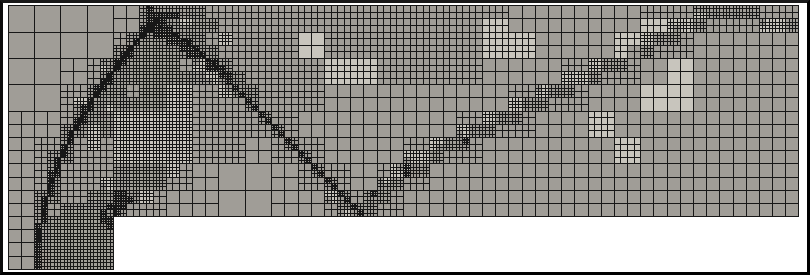
\includegraphics[width=0.7\textwidth]{examples_img/forward-step/mesh3.png}
\end{center}

\caption{Solution (Mach number distribution), and mesh, time = 2.87897.}

\label{fig:ffs-3}
\end{figure}

\begin{figure}[H]
\begin{center}
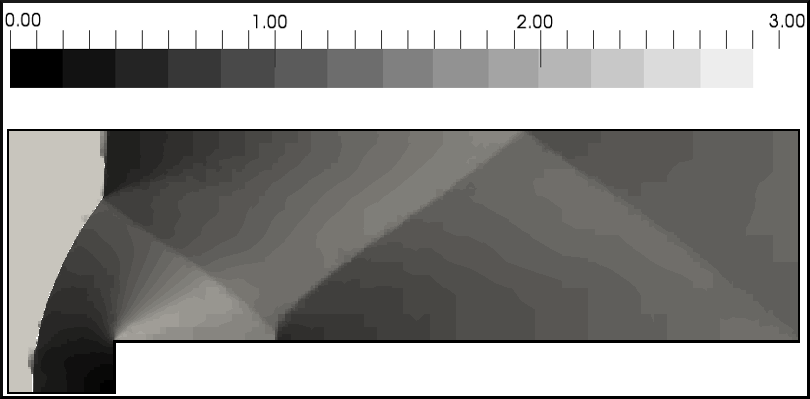
\includegraphics[width=0.7\textwidth]{examples_img/forward-step/sln4.png}\\
\vspace{2mm}
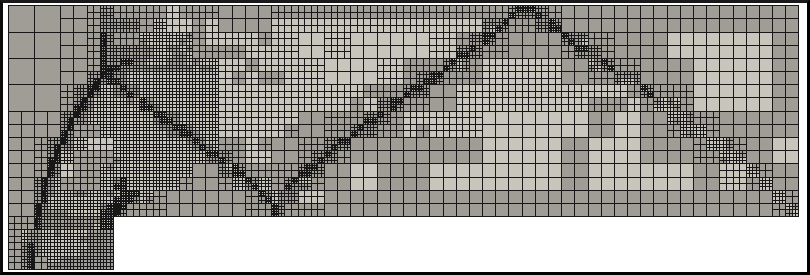
\includegraphics[width=0.7\textwidth]{examples_img/forward-step/mesh4.png}
\end{center}

\caption{Solution (Mach number distribution), and mesh, time = 3.5648.}

\label{fig:ffs-4}
\end{figure}
